\documentclass{beamer}
\usepackage[style=numeric-comp, backend=biber, giveninits=true]{biblatex}
\usepackage{lmodern}
\usepackage{amsmath}
\usepackage{mathtools}
\usepackage[version=3]{mhchem} % Formula subscripts using \ce{}, e.g., \ce{H2SO4}
\usepackage{siunitx}
\usepackage[utf8]{inputenc}

\graphicspath{{./Figures/}}
%smaller footnotes, adapted from http://tex.stackexchange.com/a/146021
\setbeamerfont{footnote}{size=\fontsize{7pt}{0pt}}

%footnote spacing avoids navigation / margins, adapted from http://tex.stackexchange.com/a/44231
\addtobeamertemplate{footnote}{\vspace{-6pt}\advance\hsize-0.5cm}{\vspace{6pt}}
\makeatletter
% Alternative A: footnote rule
\renewcommand*{\footnoterule}{\kern -3pt \hrule \@width 2in \kern 8.6pt}
% Alternative B: no footnote rule
% \renewcommand*{\footnoterule}{\kern 6pt}
\makeatother

%make frame for each section
\AtBeginSection[]{
  \begin{frame}
  \vfill
  \centering
  \begin{beamercolorbox}[sep=8pt,center,shadow=true,rounded=true]{title}
    \usebeamerfont{title}\insertsectionhead\par%
  \end{beamercolorbox}
  \vfill
  \end{frame}
}

\newcounter{dummynote1}% Save footnote counter
\newcounter{dummynote2}% Save footnote counter

\bibliography{lit_review.bib}

%opening
\title{SIMT\slash SIMD computation on CPUs and Co-processors: A Literature Review}
\author{Nick Curtis}
\institute{University of Connecticut}
\date{\today}

\begin{document}

\maketitle

\section{Introduction}

\begin{frame}
\frametitle{Chemical Kinetic Simulations are \textbf{Critical}}
In order to meet increasingly stringent emissions and efficiency requirements, designers of combustion devices have turned to \textbf{new technologies} and \textbf{new fuels}
\begin{itemize}
 \item Novel combustion regimes such as low-temperature combustion are often controlled by chemical processes, rather than directly controllable physical processes as in current technology
 \item Further, developed solutions must be flexible to accommodate a variety of next generation fuels
\end{itemize}
Computationally guided combustion design has played an important role in development of these new technologies, however use of realistic chemical modeling (as required for predictive reacting-flow simulations) is prohibitively expensive for most practical systems. 
\end{frame}

\begin{frame}
 \frametitle{Chemical Kinetic Integration is \textbf{Expensive}}
 The size of chemical kinetic models for fuels relevant transportation and energy generation may consist of hundreds to thousands of chemical species, with potentially tens of thousands of reactions.
 \begin{itemize}
  \item e.g., for gasoline \footfullcite{Mehl:2011cn} and jet fuel\footfullcite{Naik2011434}
 \end{itemize}
 Further, chemical kinetic models are typically \textbf{stiff}---due to the presence of highly reactive radicals and associated short chemical timescales.
 \begin{itemize}
  \item Typically implicit integration techniques are used to efficiently deal with stiffness, requiring repeated evaluation and factorization of the chemical kinetic Jacobian.
  \item Naive implementations of these operations scale \textbf{quadratically} and \textbf{cubically} with the number of species in a model, respectively\footfullcite{Lu:2009gh}.
 \end{itemize}
\end{frame}

\begin{frame}
 \frametitle{Strategies for cost reduction}
 A few major strategies exist to accelerate chemical kinetic integration:
 \begin{itemize}
  \item \textbf{Model reduction}, a host of techniques to reduce the size of the system being solved while maintaining accurate chemical kinetics (as compared to the full model)
  \item \textbf{Improved integration techniques}, development of new integration algorithms specifically for chemical kinetics, e.g. hybrid implicit\slash explicit integrators, tabulation techniques, analytical Jacobian codes, and on-the-fly stiffness removal
  \item \textbf{Solver vectorization}, reformulation of solvers for efficient single-instruction, multiple-data (SIMD) execution both on specialized hardware---e.g. graphics processing units (GPUs)---and modern central processing units (CPUs)
  \item \textbf{High performance computing techniques}, stiffness-based load balancing, scaling for high performance clusters
 \end{itemize}
 We will focus on \textbf{vectorization}, \texbf{novel solvers} and \textbf{high performance computing}.
\end{frame}

\begin{frame}
 \frametitle{Operator Splitting and Vectorization}
 Most reactive-flow codes utilize the operator-splitting techniques (e.g.~\footfullcite{Knio:1999}$^{,}$~\footfullcite{Ren:2008}), separating a large system of coupled partial differential equations (PDEs), such that different physical processes are solved independently.
 \begin{itemize}
  \item Stiff integration technique used for chemical kinetics, and an explicit scheme for transport, etc.
  \item Avoids the high cost of solving the fully coupled PDEs
  \item Independent system of ODEs at each computational location (e.g. cell) in the domain~$\rightarrow$~vectorization!
 \end{itemize}
 It is noted that significant error can be introduced by operator-splitting schemes if the time-steps are not chosen properly~\footfullcite{Gao2015287}.
\end{frame}

\section{Single Instruction, Multiple Data\slash Thread Processing Paradigms}

\begin{frame}
 \frametitle{Single Instruction, Multiple Data Processing}
 \begin{columns}
 
 \begin{column}{0.6\textwidth}
  \textbf{Single Instruction, Multiple Data (SIMD)} processing is a vector processing paradigm that allows processing elements (PE)---e.g a CPU core---to execute the same instruction concurrently on different data.
  \begin{itemize}
    \item Each vector unit contains multiple processing units (PUs), which are called a \textbf{lane}
    \item Each vector unit operates on a \textbf{superword}, a variable length data array---typically, \numrange{2}{16} double precision floats (doubles)
    \item Typically a single thread resides on each PE and issues SIMD vector instructions over multiple data
    %\begin{itemize}
    % \item It is possible to have multiple threads per PE, but SIMD instructions between threads do not interact
    %\end{itemize}
  \end{itemize}
 \end{column}
 \begin{column}{0.4\textwidth}
  \begin{figure}
    \centering
    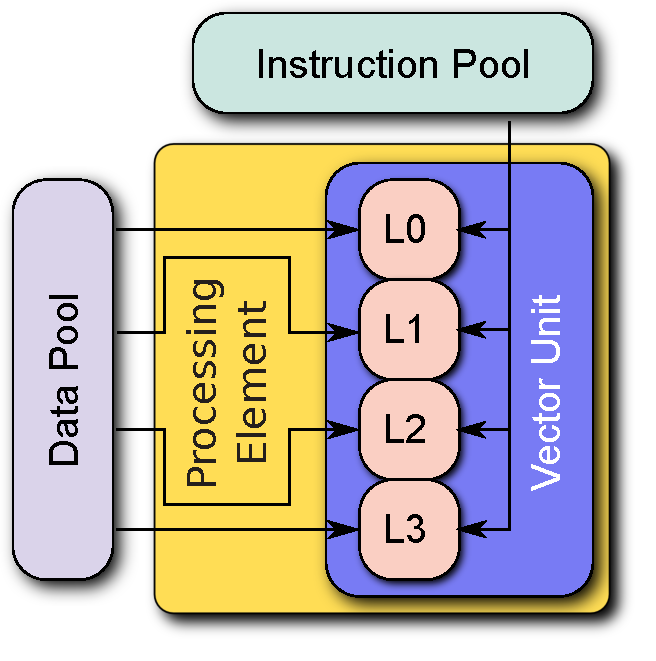
\includegraphics[width=\columnwidth]{SIMD.pdf}
    \caption{Schematic of SIMD processing.  Adapted from\footnotemark}
  \end{figure}
 \end{column}
 \footnotetext{\fullcite{Simdfig:2016}}
 \end{columns}
\end{frame}

\begin{frame}
 \frametitle{Single Instruction, Multiple Thread Processing}
 \begin{columns}
 \begin{column}{0.6\textwidth}
 \textbf{Single instruction, multiple thread (SIMT)} processing is a related, though separate concept.
 \begin{itemize}
  \item Multiple threads reside on a PE, each with instructions to execute at each step (\textrm{I1}, \textrm{I2} in the example)
  \item All threads that need to execute the same instruction (e.g. \textrm{I1}) execute simultaneously
  \item If some threads need a different instruction (e.g. \textrm{I2}), they must wait and execute their instruction after the other threads
  \item This is known as \textbf{thread divergence}, and is an important performance concern.
 \end{itemize}
 \end{column}
 \begin{column}{0.4\textwidth}
  \begin{figure}[r]
    \centering
    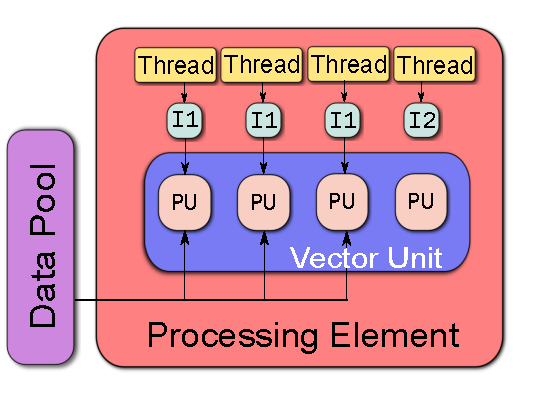
\includegraphics[width=\columnwidth]{SIMT.pdf}
    \caption{Schematic of SIMT processing}
  \end{figure}
 \end{column}
 \end{columns}
\end{frame}

    
\begin{frame}
 \frametitle{CPU-based SIMD Computing for ODE integration}
 GPUs allow easy implementation of SIMT programs, while SIMD programs are typically easier to construct for CPUs~\footfullcite{Stone:2016}.
 For CPU-based SIMD computing, different levels of parallelism are available:
 \begin{itemize}
  \item Multiple PEs (e.g. multiple cores)
  \item SIMD processing available within each PE
  \item Additionally, multiple threads may reside on PE (e.g.a \textit{hyperthreaded} CPU core)
 \end{itemize}
 Different levels of SIMD cooperation possible:
 \begin{itemize}
  \item Each set of ODEs is assigned to separate SIMD lane, meaning a thread solves multiple sets of ODEs $\rightarrow$ \textbf{shallow} vectorization
  \item Each thread uses SIMD operators to vectorize solution of a single set of ODEs $\rightarrow$ \textbf{deep} vectorization
 \end{itemize}
\end{frame}

\begin{frame}
  \frametitle{CPU-based SIMD Computing -- Difficulties}
  Explicit use of SIMD instructions is typically platform--dependent and difficult to implement\footfullcite{Stone:2016}.
  \begin{itemize}
   \item Specialized compilers are often used to identify vectorizable loops and generate the appropriate platform--dependent SIMD code.
  \end{itemize}
  Recently many tools have emerged to ease the development burden of SIMD programming
  \begin{itemize}
   \item \texttt{OpenCL}~\footfullcite{Stone:2010} is a platform--independent language geared towards SIMT\slash SIMD programming.
   \item \texttt{loo.py}~\footfullcite{Klockner:2014} is a python--based code generation platform that generates explicit SIMT\slash SIMD code for CPUs and GPUs
  \end{itemize}
\end{frame}

\section{CPU-based SIMD Integration of Stiff ODEs}

\begin{frame}
 \frametitle{Comparison of SIMD and SIMT parallelization on multiple platforms}
 Stone and Niemeyer~\footfullcite{Stone:2016} investigated the effect of both wide and deep SIMD\slash SIMT parallelization on two fourth-order-explicit integration techniques (and accompanying chemical kinetic rate evaluation subroutines) on the CPU, GPU and an Intel Xeon Phi co-processor (MIC).
 \begin{itemize}
  \item The most efficient word-size was 2--4 doubles on both the CPU and MIC
  \item Speedups of \SIrange[range-phrase=--, range-units = single]{2}{3}{\times} (over a baseline OpenMP parallelized CPU version) were achieved for chemical kinetic rate evaluation using deep-vectorized CPU\slash MIC codes, and shallow-vectorized GPU codes
  \item Speedups of up to \SI{1.4}{\times}, \SI{2.5}{\times} and \SI{3.2}{\times} were found for a stiff Rosenbrock solver for the GPU, CPU, and MIC respectively.
  \item Thread divergence may cause significant performance degradation for the GPU solvers
 \end{itemize}
\end{frame}

\begin{frame}
 \frametitle{Shallow-SIMD RODAS solver on a Cell Broadband Engine}
 Kroshko and Spiteri~\footfullcite{Kroshko:2013} implemented a fourth-order Rodenbrock solver (RODAS) capable of solving differential algebraic equations for a cell broadband engine (CBE), a hybrid CPU\slash SIMD processor.
 \begin{itemize}
  \item A shallow-SIMD program was developed using explicit SIMD instructions to model \ce{CO2} reformation on a \ce{Pd} catalyst in a plug-flow reactor.
  \item A speedup of \SI{1.89}{\times} was found over a purely serial solver.
  \item The CBE had two double precision SIMD lanes, hence the parallel efficiency: $\epsilon = \frac{1.89}{2.0} = 0.94$.
  \item The number of integrator steps taken\slash rejected, and hence thread divergence, depended strongly (but smoothly) on the initial conditions; a clustering method was suggested to pair similar IVPs to improve efficiency.
 \end{itemize}
\end{frame}

\begin{frame}
 \frametitle{Thread-divergence Mitigation for SIMD\slash SIMT-based ODE Integration}
 \only<1>
 {
 One significant source of thread-divergence for shallow SIMD\slash SIMT ODE solvers is differing time-step sizes between ODE problems
 \begin{itemize}
   \item Adaptive time-stepping strategies are commonly used to maintain accuracy while minimizing computational effort (compared to a fixed time-step)
   \item The number of adaptive time-steps required to complete integration is typically not known a priori, and may be \textit{severely} unbalanced between ODEs processed together in a SIMD\slash SIMT program
    \item This may result in significant wastage of computational cycles $\rightarrow$ \textbf{thread divergence}
 \end{itemize}
 }
 \only<2>
 {
  Murray~\footfullcite{Murray:2012} presented a method of mitigating this issue:
  \begin{itemize}
    \item Instead of lane\slash thread (work unit) solving a single set of ODEs, it was suggested to assign multiple sets of ODEs to each work unit
    \item When integration of a set of ODEs completes, the work unit immediately begins to solve the next set of ODEs
    \item This packing scheme may result in uncoalesced\slash irregular memory accesses, however:
    \begin{itemize}
     \item Analytically it approaches ideal parallel scaling
     \item Empirically a \SI{10}{\percent} improvement  was found over the non-packed version on a GPU
     \item The GPU used in this study is quite old and may have been more adversely affected by uncoalesced memory accesses than a modern GPU
    \end{itemize}
  \end{itemize}
 }
\end{frame}

\begin{frame}
 \frametitle{Automatic SIMD-enabled Code Generation for Atmospheric Chemical Kinetics}
 \setcounter{dummynote1}{\value{footnote}}
 \setcounter{dummynote2}{\value{footnote}}
 \addtocounter{dummynote1}{1}
 \addtocounter{dummynote2}{2}
 \only<1>
 {
  Linford and Sandu\footnotemark[\value{dummynote1}]~developed a framework for implementation of SIMD-enabled atmospheric chemical kinetic integration, using a Rosenbrock solver.
 \begin{itemize}
  \item All loops are completely unrolled (i.e. static code is generated)
  \item 29 different level-zero basic linear algebra subprograms (BLAS) operations were developed using SIMD-operations, resulting in up to a \SI{5}{\times} speedup
 \end{itemize}
 }
 Linford et al.\footnotemark[\value{dummynote2}]~extended this work to GPUs and CBEs.
 \begin{itemize}
  \only<1>
  {
  \item The CPU version used one OpenMP thread per computational cell, and utilized SIMD operations to accelerate source term and Jacobian evaluation\slash factorization
  \item The GPU solver was controlled by the CPU which called GPU kernels for Jacobian evaluation, LU Decomposition, etc.
  }
  \only<2>
  {
  \item<2-> A SIMD enabled serial CPU solver was \SI{2.0}{\times} and \SI{1.2}{\times} faster than the default serial CPU version for single\slash double precision respectively.
  \item<2-> The CBE had the best single precision performance---up to \SI{40.7}\times and \SI{11.5}{\times} speedup for single\slash double precision respectively---due to explicitly managed memory and large on-chip fast memory cache sizes, but was difficult to implement.
  \item<2-> The GPU solver was easy to implement, but difficult to optimize due to small on-chip memory cache sizes; a maximum speedup of \SI{13.7}{\times} and \SI{13.3}{\times} for single\slash double precision (respectively) was achieved.
  }
 \end{itemize}
 \only<1>
 {
 \footnotetext[\value{dummynote1}]{\fullcite{Linford:2009}}
 }
 \footnotetext[\value{dummynote2}]{\fullcite{Linford:2011}}
 \setcounter{footnote}{\value{dummynote2}} %restore the counter
\end{frame}

\section{Advanced Solvers}
\begin{frame}
\frametitle{Parallel Two-Step W-Methods}

 
\end{frame}





\end{document}
